\documentclass{beamer}

\title{Modelling Green Energy Conversion Networks for Generating Hydrogen Electric Vehicle Fuel}
\author{Lucas Ng}
\institute{University of Cambridge}
\date{31 July 2023}

\usepackage{eurosym}
\usepackage{amsmath} % for aligned
\usepackage{bm} % for bold math
%\usepackage{amssymb} % for \mathbb
\usefonttheme[onlymath]{serif}
\usepackage{tikz}
%\usepackage{etoolbox} % for \ifthen
\usepackage{listofitems} % for \readlist to create arrays
\usetikzlibrary{arrows.meta} % for arrow size
\usepackage[outline]{contour} % glow around text
\contourlength{1.4pt}

\tikzset{>=latex} % for LaTeX arrow head
\usepackage{xcolor}
\colorlet{myred}{red!80!black}
\colorlet{myblue}{blue!80!black}
\colorlet{mygreen}{green!60!black}
\colorlet{myyellow}{yellow!80!black}
\colorlet{myorange}{orange!70!red!60!black}
\colorlet{mydarkred}{red!30!black}
\colorlet{mydarkblue}{blue!40!black}
\colorlet{mydarkgreen}{green!30!black}
\colorlet{mydarkyellow}{yellow!40!black}
\tikzstyle{node}=[thick,circle,draw=myblue,minimum size=22,inner sep=0.5,outer sep=0.6]
\tikzstyle{node in}=[node,green!20!black,draw=mydarkgreen!30!black,fill=mygreen!25]
\tikzstyle{node hidden}=[node,blue!20!black,draw=myblue!30!black,fill=myblue!20]
\tikzstyle{node convol}=[node,orange!20!black,draw=myorange!30!black,fill=myorange!20]
\tikzstyle{node out}=[node,red!20!black,draw=myred!30!black,fill=myred!20]
\tikzstyle{connect}=[thick,mydarkblue] %,line cap=round
\tikzstyle{connect arrow}=[-{Latex[length=4,width=3.5]},thick,mydarkblue,shorten <=0.5,shorten >=1]
\tikzset{ % node styles, numbered for easy mapping with \nstyle
  node 1/.style={node in},
  node 2/.style={node hidden},
  node 3/.style={node out},
}
\usepackage[usestackEOL]{stackengine}
\usepackage{scalerel}
\usepackage{graphicx,amsmath}
\def\nstyle{int(\lay<\Nnodlen?min(2,\lay):3)} % map layer number onto 1, 2, or 3
\def\svmybf#1{\rotatebox{90}{\stretchto{\{}{#1}}}
\def\svnobf#1{}
\def\rlwd{.5pt}
\newcommand\notate[4][B]{%
  \if B#1\let\myupbracefill\svmybf\else\let\myupbracefill\svnobf\fi%
  \def\useanchorwidth{T}%
  \setbox0=\hbox{$\displaystyle#2$}%
  \def\stackalignment{c}\stackunder[-6pt]{%
    \def\stackalignment{c}\stackunder[-1.5pt]{%
      \stackunder[2pt]{\strut $\displaystyle#2$}{\myupbracefill{\wd0}}}{%
    \rule{\rlwd}{#3\baselineskip}}}{%
  \strut\kern9pt$\rightarrow$\smash{\rlap{$~\displaystyle#4$}}}%
}

% https://tex.stackexchange.com/a/432676
\logo{
\includegraphics[width=.1\textwidth]{assets/logo.jpg}\vspace*{.88\paperheight}}

\begin{document}

\frame{\titlepage}
% \begin{frame}
%     \frametitle{Sample frame title}
%     \framesubtitle{\rule{\textwidth}{1pt}}
% \end{frame}

% \begin{frame}
%     \frametitle{Background}
%     This is some text in the first frame. This is some text in the first frame. This is some text in the first frame.
% \end{frame}

\begin{frame}{What are we modelling?}
    The goal is to turn solar energy into hydrogen fuel to be used in HEVs. Here is a simple linear system for this:
    $$\overset{\text{Sun}}{\bullet} \xrightarrow[\text{PV cells}]{} \overset{\text{Battery}}{\bullet} \xrightarrow[\text{Electrolyser,\ Compressor}]{} \overset{H_{2} \text{ fuelling station}}{\bullet}$$
    Observe:
    \begin{itemize}
        \item The Sun, battery and $H_2$ fuelling station are energy \underline{stores}.
        \item The PV cells and electrolyser are energy \underline{converters}.
    \end{itemize}
    We can abstract this into a graph with:
    \begin{itemize}
        \item \textbf{Vertices} representing energy stores.
        \item \textbf{Edges} representing energy converters.
    \end{itemize}
\end{frame}

\begin{frame}{A more complex example}
    \begin{center}
        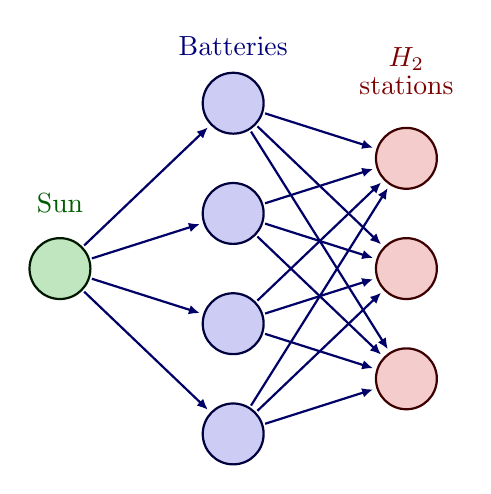
\begin{tikzpicture}[x=2.2cm,y=1.4cm]
            % Adapted from https://tikz.net/neural_networks/
            \message{^^JNeural network with arrows}
            \readlist\Nnod{1,4,3} % array of number of nodes per layer
            \message{^^J  Layer}
            \foreachitem \N \in \Nnod{ % loop over layers
                \edef\lay{\Ncnt} % alias of index of current layer
                \message{\lay,}
                \pgfmathsetmacro\prev{int(\Ncnt-1)} % number of previous layer
                \foreach \i [evaluate={\y=\N/2-\i; \x=\lay; \n=\nstyle;}] in {1,...,\N}{ % loop over nodes
                        % NODES
                        \node[node \n] (N\lay-\i) at (\x,\y){}; %{$u_\i^{(\prev)}$};
                        % CONNECTIONS
                        \ifnum\lay>1 % connect to previous layer
                            \foreach \j in {1,...,\Nnod[\prev]}{ % loop over nodes in previous layer
                                    \draw[connect arrow] (N\prev-\j) -- (N\lay-\i); % connect arrows directly
                                }
                        \fi % else: nothing to connect first layer
                    }
            }
            % LABELS
            \node[above=5,align=center,mygreen!60!black] at (N1-1.90) {Sun};
            \node[above=2,align=center,myblue!60!black] at (N2-1.90) {Batteries};
            \node[above=8,align=center,myred!60!black] at (N\Nnodlen-1.90) {$H_2$\\[-0.2em]stations};

        \end{tikzpicture}
    \end{center}
    If this sort of generalised, extensible and extendable approach is consistently taken, it is more useful for future investigation.
\end{frame}

\begin{frame}{Theory}
    Begin with some definitions:
    \begin{itemize}
        \item $\mathcal{V}$ is the set of vertices mapped to energy stores
        \item $\mathcal{E}$ is the set of edges mapped to energy converters
        \item $G \triangleq(\mathcal{V},\mathcal{E})\ni\mathcal{E}\subseteq\left \{(x,y):(x,y)\in\mathcal{V}^2\ \text{and}\ x\neq y\right \}$
        \item $N$ is the cardinality of $\mathcal{V}$.
        \item $\underline{\underline{A_w}}\ni \forall v_i \in \mathcal{V}, \nexists j:\left [ \sum_{k = 1}^{N} \left (\underline{\underline{A_w}}+\underline{\underline{A_w}}^\top\right )^k\right ]_{ij}= 0$ is $G$'s weighted adjacency matrix.
    \end{itemize}
    \bigbreak
    Hence the graph $G$ is defined to be simple, directed and weakly connected. Normalised edge weights $\in [0, 1]$ are used to proportion power transfer ratios.
    \bigbreak
    Non-simple networks can be modelled by edge subdivisions or adjusting edge weights.
\end{frame}

\begin{frame}{Ideal behaviour}
    Consider a single vertex with energy value $u_{i}$.
    $$\xrightarrow[\text{Net power in}]{}\overset{u_i}{\bullet} \xrightarrow[\text{Net power out}]{}$$
    Ignoring all constraints causes immediate energy propagation to and from all neighbours.
    \bigbreak
    During time-step $\varDelta t$:
    $$\varDelta u_i = -\overbrace{\sum_{j=1}^{N} \underline{\underline{A_w}}_{ij} u_i}^{\text{energy out}} +\underbrace{\sum_{j=1}^{N} \underline{\underline{A_w}}_{ji} u_j}_{\text{energy in}}$$
    $\forall\underline{\underline{A_w}},\forall\underline{u}:\sum_{i=1}^{N}\varDelta u_i=0\therefore$ this operator conserves energy.
\end{frame}

\begin{frame}{Non-ideal behaviour}
    We have the following non-idealities:
    \begin{itemize}
        \item \textbf{Vertex maximum capacity}: $u_{i_{max}} \ni 0\leq u_{i} \leq u_{i_{max}}$.
        \item \textbf{Edge maximum power transfer}: $\underline{\underline{P}}_{ij} \ni \underline{\underline{A_w}}_{ij} u_i \leq \underline{\underline{P}}_{ij} \varDelta t$ where $\underline{\underline{P}}_{ij}$ is the maximum power transfer from $i$ to $j$.
        \item \textbf{Vertex self-discharge}: loss of energy stored over time.
        \item \textbf{Edge process inefficiency}: losses during power conversion.
    \end{itemize}
    Ignore the last two for now. We can then apply the remaining constraints to the previous equation:
    $$
        \varDelta u_i = \min \left( u_{i_{\mathrm{max}}}-u_i, \begin{aligned}
             & -\sum_{j=1}^{N} \min (\underline{\underline{A_w}}_{ij} u_i, \underline{\underline{P}}_{ij} \varDelta t) \\
             & +\sum_{j=1}^{N} \min (\underline{\underline{A_w}}_{ji} u_j, \underline{\underline{P}}_{ji} \varDelta t)
        \end{aligned} \right)
    $$
\end{frame}
\begin{frame}{What about power losses?}
    Consider an arbitrary energy conversion $p_{xy}$ with efficiency $\eta_p$.
    $$\overset{x}{\bullet}\xrightarrow{\qquad p_{xy},\ \eta_p = 1\qquad}\overset{y}{\bullet}$$
    If $p$ is not, in fact, ideal, then we can model this by partitioning some power off into an energy wastage sink.
    Let's suppose it is 70\% efficient:
    $$
        \begin{aligned}
             & \overset{x}{\bullet}\ \xrightarrow{\qquad p_{xy},\ \eta_p=70\%\qquad}\overset{y}{\bullet} \\
             & \rotatebox[origin=c]{270}{$\xrightarrow{\quad 30\%\quad}$}                                \\
             & \bullet_{\ \mathrm{energy\ sink}}
        \end{aligned}
    $$
    To handle self-discharge losses, increase the weight of the edges connecting vertices to the sink.
\end{frame}

\begin{frame}{Demo: a simple linear system}
    Studying the simple linear system from earlier to demonstrate the model:
    $$\overset{\text{Sun}}{\bullet} \xrightarrow[\text{PV cells}]{} \overset{\text{Battery}}{\bullet} \xrightarrow[\text{Electrolyser,\ Compressor}]{} \overset{H_{2} \text{ fuelling station}}{\bullet}$$
    \bigbreak
    Reasonable assumptions about component behaviour and economics and solar power input over the course of a representative year were used.
    \bigbreak
    Geography-dependent data was sampled for Cyprus.
\end{frame}

\begin{frame}{Results: minimum budget to support HEVs}
    \textbf{L-BFGS-B optimisation} was used to minimise the total budget required to sustain the system:
    \begin{center}
        \begin{tabular}{|c|c|c|c|}
            \hline
            \# HEVs & Min. budget (\euro{}) & Solution $\eta$ & PV capacity (kW) \\
            \hline
            1       & 70.8k                 & 0.55            & 4.6              \\
            10      & 715k                  & 0.55            & 46               \\
            100     & 6800k                 & 0.55            & 460              \\
            \hline
        \end{tabular}
    \end{center}
    It was not possible to simulate 1000 HEVs due to constraints from the PV data API.
\end{frame}


% \begin{frame}{Results: max. HEVs supported by a given budget}
%     The following results were obtained by \textbf{Nelder-Mead optimisation}:
%     \begin{center}
%         \begin{tabular}{|c|c|c|c|c|}
%             \hline
%             \# HEVs & Min. budget (\euro{}) & Budget ratio & $\eta$ & PV (kW) \\
%             \hline
%             1       & 100                   & 90           & 90\%   & 1000    \\
%             10      & 90                    & 80           & 90\%   & 1000    \\
%             100     & 80                    & 70           & 90\%   & 1000    \\
%             1000    & 70                    & 60           & 90\%   & 1000    \\
%             \hline
%         \end{tabular}
%     \end{center}
% \end{frame}
% 645223.4719163576,
%     243960.66318646292,
%     106915.50432184557,
%     3900.360575333828,
\begin{frame}{Results: optimising given budget}
    For \euro{1M}, use \textbf{L-BFGS-B optimisation} to find the optimal budget allocation that maximises the number of HEVs supported:
    \begin{center}
        \begin{tabular}{|c|c|c|c|}
            \hline
            PV  (\euro{}) & Battery (\euro{}) & Electrolyser (\euro{}) & $H_2$ station (\euro{}) \\
            \hline
            645k          & 244k              & 107k                   & 3.90k                   \\
            \hline
        \end{tabular}
        \begin{figure}
            \centering
            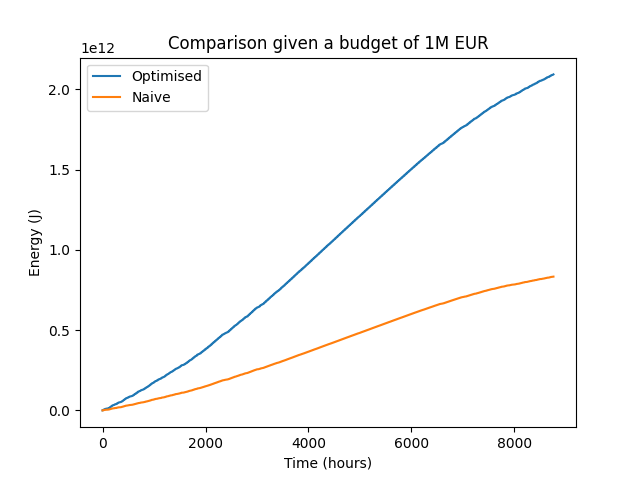
\includegraphics[width=0.75\textwidth]{assets/opt_naive_cmp.png}
        \end{figure}
    \end{center}
    % \begin{columns}[c]
    %     \begin{column}{.6\textwidth}
    %         \begin{figure}
    %             \centering
    %             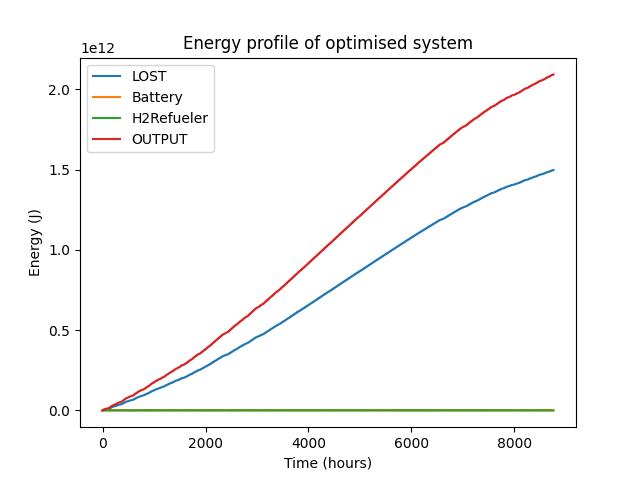
\includegraphics[width=\textwidth]{assets/opt_budget_profile.png}
    %         \end{figure}
    %     \end{column}
    %     \begin{column}{.6\textwidth}
    %     \end{column}
    % \end{columns}
\end{frame}
\begin{frame}{Results: optimising given budget (cont.)}
    \begin{center}
        \begin{figure}
            \centering
            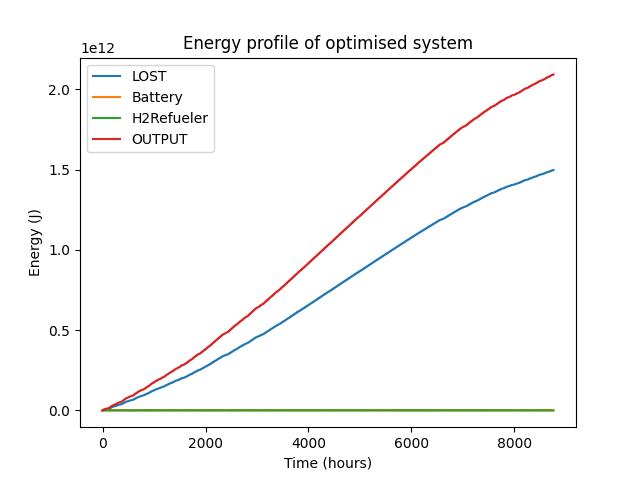
\includegraphics[width=\textwidth]{assets/opt_budget_profile.png}
        \end{figure}
    \end{center}
\end{frame}

\begin{frame}{Future potential}
    \begin{itemize}
        \item \textbf{More accurate modelling} of component behaviour, e.g. using characterisations dependent on more parameters.
        \item \textbf{Expand components into sub-networks} to give a more detailed analysis.
        \item \textbf{Investigate larger networks}, e.g. a potential national PV-HEV grid.
    \end{itemize}
\end{frame}

\end{document}